\chapter{Fonction Logarithme Népérien}

Ce chapitre présente la fonction logarithme népérien, notée $\ln$. Historiquement introduite pour simplifier les calculs astronomiques et de navigation en transformant les produits en sommes, elle joue aujourd'hui un rôle central dans toutes les sciences et en analyse mathématique.

\section{Définition et Propriétés Algébriques}

\subsection{Définition}

La fonction exponentielle est continue et strictement croissante sur $\R$, à valeurs dans $]0, +\infty[$. D'après le corollaire du théorème des valeurs intermédiaires, pour tout réel $x > 0$, l'équation $e^y = x$ d'inconnue $y$ admet une unique solution sur $\R$.

\begin{definition}[Fonction Logarithme Népérien]
On appelle **fonction logarithme népérien**, notée $\ln$, la fonction qui, à tout réel $x \in ]0, +\infty[$, associe l'unique solution $y$ de l'équation $e^y = x$.
Ainsi, pour tout $x \in ]0, +\infty[$ et tout $y \in \R$ :
\[
y = \ln(x) \iff e^y = x
\]
\end{definition}

\begin{propriete}[Relations fondamentales]
De cette définition, on déduit immédiatement :
\begin{itemize}
    \item Pour tout $x \in ]0, +\infty[$ : $e^{\ln(x)} = x$.
    \item Pour tout $y \in \R$ : $\ln(e^y) = y$.
    \item En particulier : $\ln(1) = 0$ et $\ln(e) = 1$ (où $e \approx 2,718$).
\end{itemize}
\end{propriete}

\subsection{Propriétés algébriques}

La propriété fondamentale de la fonction logarithme est de transformer les produits en sommes :

\begin{propriete}[Relation fonctionnelle et extensions]
Pour tous réels $a > 0$ et $b > 0$ :
\[
\ln(a \times b) = \ln(a) + \ln(b)
\]
On en déduit également les propriétés suivantes pour tous réels $a > 0$, $b > 0$ et $n \in \Z$ :
\begin{itemize}
    \item \textbf{Inverse} : $\ln\left(\frac{1}{a}\right) = -\ln(a)$
    \item \textbf{Quotient} : $\ln\left(\frac{a}{b}\right) = \ln(a) - \ln(b)$
    \item \textbf{Puissance} : $\ln(a^n) = n \ln(a)$
    \item \textbf{Racine carrée} : $\ln(\sqrt{a}) = \frac{1}{2} \ln(a)$
\end{itemize}
\end{propriete}

\section{Étude de la fonction logarithme}

\subsection{Variations et dérivabilité}

\begin{theoreme}[Dérivée et variations]
La fonction $\ln$ est continue et dérivable sur $]0, +\infty[$. Pour tout $x \in ]0, +\infty[$ :
\[
\ln'(x) = \frac{1}{x}
\]
Comme $x > 0$, $\ln'(x) > 0$. Ainsi, la fonction $\ln$ est **strictement croissante** sur $]0, +\infty[$.
\end{theoreme}

\begin{propriete}[Signe du logarithme]
\begin{itemize}
    \item Si $0 < x < 1$, alors $\ln(x) < 0$.
    \item Si $x > 1$, alors $\ln(x) > 0$.
\end{itemize}
\end{propriete}

\subsection{Limites aux bornes}

\begin{propriete}[Limites de référence]
\begin{itemize}
    \item En $+\infty$ : $\lim_{x \to +\infty} \ln(x) = +\infty$
    \item En $0$ (par valeurs supérieures) : $\lim_{x \to 0^+} \ln(x) = -\infty$
\end{itemize}
\textit{Conséquence géométrique} : L'axe des ordonnées (d'équation $x=0$) est une asymptote verticale à la courbe représentative de la fonction $\ln$.
\end{propriete}

\subsection{Symétrie et Représentation Graphique}

Puisque les fonctions $\ln$ et $\exp$ sont réciproques l'une de l'autre, leurs courbes représentatives dans un repère orthonormé sont symétriques par rapport à la droite d'équation $y=x$.

\begin{center}
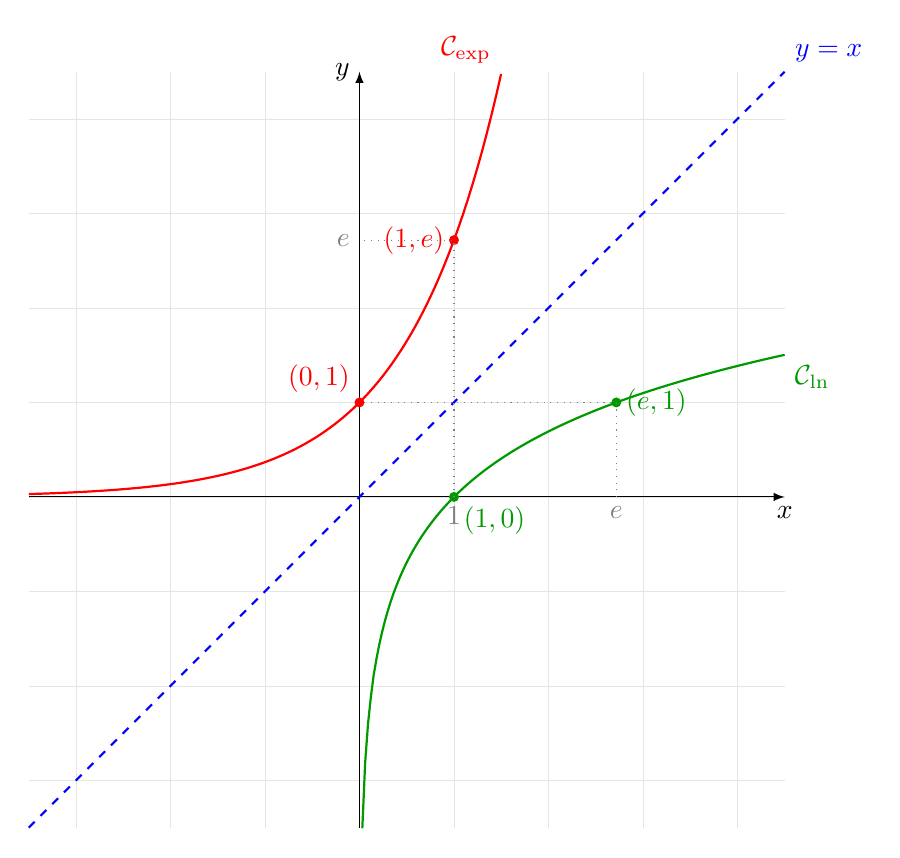
\begin{tikzpicture}[scale=1.2]
  % Grille
  \draw[gray!20,very thin] (-3.5,-3.5) grid (4.5,4.5);
  % Axes
  \draw[->,>=latex] (-3.5,0) -- (4.5,0) node[below] {$x$};
  \draw[->,>=latex] (0,-3.5) -- (0,4.5) node[left] {$y$};
  
  % Bissectrice y = x
  \draw[dashed, blue, thick] (-3.5,-3.5) -- (4.5,4.5) node[above right] {$y=x$};
  
  % Courbe exp
  \draw[domain=-3.5:1.5, samples=100, color=red, thick] plot (\x, {exp(\x)}) node[above left] {$\mathcal{C}_{\exp}$};
  
  % Courbe ln
  \draw[domain=0.03:4.5, samples=150, color=green!60!black, thick] plot (\x, {ln(\x)}) node[below right] {$\mathcal{C}_{\ln}$};
  
  % Points clés
  \fill[green!60!black] (1,0) circle (1.5pt) node[below right] {$(1,0)$};
  \fill[red] (0,1) circle (1.5pt) node[above left] {$(0,1)$};
  \fill[green!60!black] (2.718,1) circle (1.5pt) node[right] {$(e,1)$};
  \fill[red] (1,2.718) circle (1.5pt) node[left] {$(1,e)$};
  
  \draw[dotted, gray] (2.718,0) node[below] {$e$} -- (2.718,1) -- (0,1);
  \draw[dotted, gray] (1,0) node[below] {$1$} -- (1,2.718) -- (0,2.718) node[left] {$e$};
\end{tikzpicture}
\end{center}

\section{Limites de Croissances Comparées}

À l'infini, la fonction exponentielle l'emporte sur toutes les puissances de $x$, qui elles-mêmes l'emportent sur la fonction logarithme.

\begin{theoreme}[Croissances comparées pour $\ln$]
Pour tout entier naturel $n \ge 1$ :
\[
\lim_{x \to +\infty} \frac{\ln(x)}{x^n} = 0 \quad \text{et} \quad \lim_{x \to 0^+} x^n \ln(x) = 0
\]
\end{theoreme}

\section{Méthodes Clés}

\begin{methode}[Résoudre des équations et inéquations avec $\ln$]
Pour résoudre une équation ou une inéquation contenant des logarithmes :
\begin{enumerate}
    \item **Déterminer le domaine d'étude** : les expressions situées dans chaque logarithme doivent être strictement positives.
    \item **Simplifier les expressions** à l'aide des formules algébriques pour regrouper les logarithmes sous la forme $\ln(A) = \ln(B)$ ou $\ln(A) < \ln(B)$.
    \item **Utiliser la stricte croissance** de la fonction $\ln$ :
    \[
    \ln(A) = \ln(B) \iff A = B \quad \text{et} \quad \ln(A) < \ln(B) \iff A < B
    \]
    \item **Vérifier** que les solutions trouvées appartiennent au domaine d'étude.
\end{enumerate}
\end{methode}

\begin{exemple}[Résolution d'inéquation]
Résolvons dans $\R$ l'inéquation : $\ln(x-1) + \ln(x) \le \ln(2)$.
\begin{enumerate}
    \item **Domaine d'étude** : On doit avoir $x-1 > 0$ et $x > 0$, c'est-à-dire $x > 1$. L'ensemble d'étude est donc $D = ]1, +\infty[$.
    \item **Simplification** : Pour $x \in D$, $\ln(x-1) + \ln(x) = \ln(x(x-1)) = \ln(x^2-x)$. L'inéquation devient :
    \[
    \ln(x^2-x) \le \ln(2) \iff x^2 - x \le 2 \iff x^2 - x - 2 \le 0
    \]
    Le discriminant du trinôme est $\Delta = (-1)^2 - 4(1)(-2) = 9 > 0$. Les racines sont $x_1 = -1$ et $x_2 = 2$.
    Le trinôme est négatif ou nul entre ses racines, c'est-à-dire sur $[-1, 2]$.
    \item **Conclusion** : En croisant avec l'ensemble d'étude $D = ]1, +\infty[$, on obtient l'ensemble des solutions :
    \[
    S = ]1, 2]
    \]
\end{enumerate}
\end{exemple}

\section{Exercices d'Entraînement Résolus}

\subsection*{Exercice 1 : Équation logarithmique simple}
Résoudre dans $\R$ l'équation suivante :
\[
\ln(2x - 1) = 3
\]

\textbf{Solution :}
1. **Domaine d'étude** : L'expression sous le logarithme doit être strictement positive :
   \[
   2x - 1 > 0 \iff x > \frac{1}{2} \implies D = \left] \frac{1}{2}, +\infty \right[
   \]
2. **Résolution** :
   \[
   \ln(2x - 1) = 3 \iff 2x - 1 = e^3 \iff 2x = e^3 + 1 \iff x = \frac{e^3 + 1}{2}
   \]
3. **Vérification** : Comme $e^3 > 0$, $\frac{e^3 + 1}{2} > \frac{1}{2}$, la solution appartient bien à $D$.
L'ensemble des solutions est :
\[
S = \left\{ \frac{e^3 + 1}{2} \right\}
\]

\subsection*{Exercice 2 : Inéquation logarithmique}
Résoudre dans $\R$ l'inéquation suivante :
\[
\ln(x^2 - 1) \ge \ln(3)
\]

\textbf{Solution :}
1. **Domaine d'étude** : On doit avoir $x^2 - 1 > 0 \iff x^2 > 1 \iff x \in ]-\infty, -1[ \cup ]1, +\infty[ = D$.
2. **Résolution** : Par stricte croissance de la fonction $\ln$ sur $]0, +\infty[$ :
   \[
   \ln(x^2 - 1) \ge \ln(3) \iff x^2 - 1 \ge 3 \iff x^2 \ge 4 \iff x \in ]-\infty, -2] \cup [2, +\infty[
   \]
3. **Vérification** : L'ensemble obtenu est entièrement inclus dans le domaine d'étude $D$.
L'ensemble des solutions est :
\[
S = ]-\infty, -2] \cup [2, +\infty[
\]

\subsection*{Exercice 3 : Limite par croissance comparée}
Déterminer la limite en $+\infty$ de la fonction $f$ définie sur $]0, +\infty[$ par :
\[
f(x) = \frac{\ln(x)}{x^2}
\]

\textbf{Solution :}
C'est une forme indéterminée du type « $\frac{\infty}{\infty}$ ».
D'après le théorème des croissances comparées, pour tout entier $n \ge 1$, $\lim_{x \to +\infty} \frac{\ln(x)}{x^n} = 0$.
En choisissant $n = 2$, on obtient directement :
\[
\lim_{x \to +\infty} f(x) = 0
\]

\subsection*{Exercice 4 : Limite en 0 par croissance comparée}
Déterminer la limite en $0^+$ de la fonction $f$ définie sur $]0, +\infty[$ par :
\[
f(x) = x \ln(x)
\]

\textbf{Solution :}
C'est une forme indéterminée du type « $0 \times (-\infty)$ ».
D'après le cours, le théorème des croissances comparées en $0^+$ énonce que pour tout $n \ge 1$ :
\[
\lim_{x \to 0^+} x^n \ln(x) = 0
\]
En posant $n = 1$, on obtient :
\[
\lim_{x \to 0^+} f(x) = 0
\]

\subsection*{Exercice 5 : Limite de quotient sans indétermination}
Déterminer la limite en $0^+$ de la fonction $f$ définie sur $]0, +\infty[$ par :
\[
f(x) = \frac{\ln(x)}{x}
\]

\textbf{Solution :}
Étudions séparément la limite du numérateur et du dénominateur :
- $\lim_{x \to 0^+} \ln(x) = -\infty$.
- $\lim_{x \to 0^+} \frac{1}{x} = +\infty$.
Puisque $f(x) = \ln(x) \times \frac{1}{x}$, par produit de limites (« $-\infty \times (+\infty)$ ») :
\[
\lim_{x \to 0^+} f(x) = -\infty
\]
Il n'y avait pas d'indétermination ici.

\subsection*{Exercice 6 : Dérivation d'un logarithme composé}
Déterminer la dérivée de la fonction $f$ définie sur $]1, 2[$ par :
\[
f(x) = \ln(-x^2 + 3x - 2)
\]

\textbf{Solution :}
La fonction $f$ est de la forme $\ln(u)$ avec $u(x) = -x^2 + 3x - 2$.
Pour $x \in ]1, 2[$, le trinôme $u(x)$ est strictement positif (car ses racines sont 1 et 2, et le coefficient devant $x^2$ est négatif). La fonction est donc dérivable.
Sa dérivée est $u'(x) = -2x + 3$.
D'après la formule $(\ln(u))' = \frac{u'}{u}$, on obtient :
\[
f'(x) = \frac{-2x + 3}{-x^2 + 3x - 2}
\]

\subsection*{Exercice 7 : Équation de type second degré en $\ln(x)$}
Résoudre dans $]0, +\infty[$ l'équation suivante :
\[
(\ln(x))^2 - 3\ln(x) + 2 = 0
\]

\textbf{Solution :}
Posons le changement de variable $X = \ln(x)$. L'équation devient :
\[
X^2 - 3X + 2 = 0
\]
C'est une équation du second degré. Le discriminant est $\Delta = (-3)^2 - 4(1)(2) = 1 > 0$.
Les solutions pour $X$ sont :
\[
X_1 = \frac{3-1}{2} = 1 \quad \text{et} \quad X_2 = \frac{3+1}{2} = 2
\]
Revenons à la variable $x$ :
- $\ln(x) = 1 \iff x = e^1 = e$.
- $\ln(x) = 2 \iff x = e^2$.
Les deux solutions appartiennent bien au domaine $]0, +\infty[$.
L'ensemble des solutions est :
\[
S = \{e; e^2\}
\]

\subsection*{Exercice 8 : Limite par factorisation forcée}
Déterminer la limite en $+\infty$ de la fonction $f$ définie sur $]0, +\infty[$ par :
\[
f(x) = \ln(x) - x
\]

\textbf{Solution :}
C'est une forme indéterminée du type « $\infty - \infty$ ». Facteur commun $x$ :
\[
f(x) = x \left( \frac{\ln(x)}{x} - 1 \right)
\]
D'après les croissances comparées, $\lim_{x \to +\infty} \frac{\ln(x)}{x} = 0$.
Le terme dans la parenthèse tend donc vers $0-1 = -1$.
Par produit de limites (« $+\infty \times (-1)$ ») :
\[
\lim_{x \to +\infty} f(x) = -\infty
\]

\subsection*{Exercice 9 : Équation de tangente}
Déterminer l'équation de la droite tangente $\mathcal{T}_e$ à la courbe de la fonction logarithme $f(x) = \ln(x)$ au point d'abscisse $x=e$.

\textbf{Solution :}
L'équation de la tangente en $a = e$ est :
\[
y = f'(e)(x-e) + f(e)
\]
On sait que $f(e) = \ln(e) = 1$.
De plus, $f'(x) = \frac{1}{x}$, donc $f'(e) = \frac{1}{e}$.
L'équation de la tangente est donc :
\[
y = \frac{1}{e}(x-e) + 1 \implies y = \frac{1}{e}x - 1 + 1 \implies y = \frac{1}{e}x
\]

\subsection*{Exercice 10 : Domaine de définition}
Déterminer le domaine de définition de la fonction $g$ définie par :
\[
g(x) = \ln\left( \frac{x-1}{2-x} \right)
\]

\textbf{Solution :}
La fonction logarithme n'est définie que pour des valeurs strictement positives. On doit donc résoudre l'inéquation :
\[
\frac{x-1}{2-x} > 0
\]
Dresseur un tableau de signes pour ce quotient :
- Le numérateur $x-1$ s'annule en $x=1$ et est positif pour $x > 1$.
- Le dénominateur $2-x$ s'annule en $x=2$ (valeur interdite) et est positif pour $x < 2$.
Le quotient est donc strictement positif entre les valeurs 1 et 2.
Le domaine de définition de $g$ est :
\[
D_g = ]1, 2[
\]

\section{Problèmes Résolus}

\subsection*{Problème 1 : Étude de la fonction $f(x) = x - \ln(x)$}
Soit la fonction $f$ définie sur $]0, +\infty[$ par :
\[
f(x) = x - \ln(x)
\]
On note $\mathcal{C}_f$ sa courbe représentative.
\begin{enumerate}
    \item Déterminer les limites de $f$ aux bornes de son domaine de définition.
    \item Calculer la dérivée $f'(x)$ et étudier les variations de $f$.
    \item En déduire le signe de $f(x)$ sur $]0, +\infty[$. Que peut-on en déduire pour les positions relatives de la courbe $\mathcal{C}_f$ et de la droite d'équation $y = \ln(x)$ ? (Non, plutôt comparer $x$ et $\ln(x)$).
    \item Démontrer que pour tout $x > 0$, $\ln(x) < x$.
    \item Étudier la convexité de $f$ sur $]0, +\infty[$.
\end{enumerate}

\textbf{Solution :}
\begin{enumerate}
    \item - Limite en $0^+$ : $\lim_{x \to 0^+} x = 0$ et $\lim_{x \to 0^+} -\ln(x) = +\infty$. Par somme, $\lim_{x \to 0^+} f(x) = +\infty$.
      - Limite en $+\infty$ : C'est une forme indéterminée. Factourisons par $x$ :
      \[
      f(x) = x \left( 1 - \frac{\ln(x)}{x} \right)
      \]
      Comme $\lim_{x \to +\infty} \frac{\ln(x)}{x} = 0$, le terme dans la parenthèse tend vers 1. Par produit, $\lim_{x \to +\infty} f(x) = +\infty$.
      
    \item La fonction $f$ est dérivable sur $]0, +\infty[$ :
      \[
      f'(x) = 1 - \frac{1}{x} = \frac{x-1}{x}
      \]
      Comme $x > 0$, $f'(x)$ a le même signe que $x-1$.
      - $f'(x) < 0$ sur $]0, 1[$, donc $f$ est strictement décroissante sur $]0, 1]$.
      - $f'(x) > 0$ sur $]1, +\infty[$, donc $f$ est strictement croissante sur $[1, +\infty[$.
      - $f'(x) = 0 \iff x = 1$.
      Le minimum global de $f$ est $f(1) = 1 - \ln(1) = 1$.
      
    \item Puisque le minimum de $f$ sur $]0, +\infty[$ est 1, on en déduit que pour tout $x \in ]0, +\infty[$ :
      \[
      f(x) \ge 1 > 0
      \]
      La fonction $f$ est donc strictement positive sur son domaine.
      
    \item Puisque $f(x) > 0 \implies x - \ln(x) > 0 \implies \ln(x) < x$ pour tout $x \in ]0, +\infty[$.
    
    \item Calculons la dérivée seconde :
      \[
      f''(x) = \left( 1 - \frac{1}{x} \right)' = \frac{1}{x^2}
      \]
      Pour tout $x > 0$, $f''(x) > 0$. La fonction $f$ est donc strictement convexe sur $]0, +\infty[$.
\end{enumerate}

\subsection*{Problème 2 : Étude de la fonction $f(x) = \frac{\ln(x)}{x}$}
Soit la fonction $f$ définie sur $]0, +\infty[$ par :
\[
f(x) = \frac{\ln(x)}{x}
\]
\begin{enumerate}
    \item Déterminer les limites de $f$ en 0 et en $+\infty$. Préciser les asymptotes à la courbe $\mathcal{C}_f$.
    \item Calculer la dérivée $f'(x)$ et en déduire les variations de $f$. Dresser le tableau de variations complet.
    \item Déterminer l'équation de la tangente $\mathcal{T}$ au point d'abscisse 1.
    \item En utilisant la convexité ou l'étude de la fonction $g(x) = \ln(x) - x + 1$ (dont on admet que $g(x) \le 0$), étudier la position de la courbe $\mathcal{C}_f$ par rapport à sa tangente $\mathcal{T}$.
\end{enumerate}

\textbf{Solution :}
\begin{enumerate}
    \item - Limite en $0^+$ : $\lim_{x \to 0^+} \ln(x) = -\infty$ et $\lim_{x \to 0^+} \frac{1}{x} = +\infty$. Par produit, $\lim_{x \to 0^+} f(x) = -\infty$.
      L'axe des ordonnées ($x=0$) est une asymptote verticale à la courbe $\mathcal{C}_f$.
      - Limite en $+\infty$ : Par croissance comparée, $\lim_{x \to +\infty} \frac{\ln(x)}{x} = 0$.
      La droite d'équation $y=0$ (l'axe des abscisses) est une asymptote horizontale à la courbe $\mathcal{C}_f$ en $+\infty$.
      
    \item La fonction $f$ est dérivable sur $]0, +\infty[$ :
      \[
      f'(x) = \frac{\frac{1}{x} \cdot x - \ln(x) \cdot 1}{x^2} = \frac{1 - \ln(x)}{x^2}
      \]
      Comme $x^2 > 0$, le signe de $f'(x)$ est celui de $1-\ln(x)$.
      - $1 - \ln(x) > 0 \iff \ln(x) < 1 \iff x < e$.
      La fonction $f$ est donc strictement croissante sur $]0, e]$ et strictement décroissante sur $[e, +\infty[$.
      Le maximum de $f$ est atteint en $x = e$ et vaut $f(e) = \frac{\ln(e)}{e} = \frac{1}{e} \approx 0,368$.
      
    \item L'équation de la tangente en 1 est :
      \[
      y = f'(1)(x-1) + f(1)
      \]
      On a $f(1) = \frac{\ln(1)}{1} = 0$ et $f'(1) = \frac{1-\ln(1)}{1^2} = 1$.
      L'équation de la tangente est donc :
      \[
      \mathcal{T} : \quad y = x - 1
      \]
      
    \item Étudions la différence $f(x) - (x-1) = \frac{\ln(x) - x(x-1)}{x} = \frac{\ln(x) - x^2 + x}{x}$.
      Cette différence est complexe à étudier directement. Mais on peut utiliser l'inégalité de la tangente pour la fonction $\ln$ : on sait que la fonction $\ln$ est concave, sa courbe est donc en dessous de sa tangente en 1 d'équation $y = x-1$.
      Donc pour tout $x > 0$, $\ln(x) \le x - 1$.
      Puisque $x > 0$, en divisant par $x$ :
      \[
      \frac{\ln(x)}{x} \le \frac{x-1}{x} = 1 - \frac{1}{x}
      \]
      Or, pour tout $x \in ]0, +\infty[$, on a l'inégalité $1 - \frac{1}{x} < x - 1$ (car $1 - \frac{1}{x} - (x - 1) = -\frac{(x-1)^2}{x} \le 0$).
      Donc $\frac{\ln(x)}{x} \le x-1$.
      La courbe $\mathcal{C}_f$ est située en dessous de sa tangente $\mathcal{T}$ en 1 pour tout $x \in ]0, +\infty[$.
\end{enumerate}

\subsection*{Problème 3 : Famille de fonctions $f_n(x) = x^n \ln(x)$}
Pour tout entier naturel $n \ge 1$, on considère la fonction $f_n$ définie sur $]0, +\infty[$ par :
\[
f_n(x) = x^n \ln(x)
\]
On note $\mathcal{C}_n$ la courbe représentative de $f_n$.
\begin{enumerate}
    \item Démontrer que toutes les courbes $\mathcal{C}_n$ passent par deux points fixes $A$ et $B$ dont on déterminera les coordonnées.
    \item Déterminer les limites de $f_n$ aux bornes de son domaine de définition (pour la limite en $0^+$, on utilisera une croissance comparée).
    \item Calculer la dérivée $f_n'(x)$ et étudier les variations de $f_n$.
    \item Dresser le tableau de variations complet de $f_n$.
\end{enumerate}

\textbf{Solution :}
\begin{enumerate}
    \item Cherchons les points fixes en résolvant $f_n(x) = f_{n+1}(x)$ :
    \[
    x^n \ln(x) = x^{n+1} \ln(x) \iff x^n \ln(x) (1-x) = 0
    \]
    Puisque $x > 0$, cela équivaut à $\ln(x) = 0$ ou $1-x = 0$, soit $x = 1$ ou $x = 1$ (qui donne la même chose) ou le point limite.
    En fait, évaluons en $x=1$ et $x$ tendant vers 0 ou autre point. Les valeurs de $x$ pour lesquelles $f_n(x)$ ne dépend pas de $n$ :
    - Si $x = 1$, $f_n(1) = 1^n \ln(1) = 0$. Le point fixe est $A(1, 0)$.
    - De plus, si on considère l'expression, elle s'annule ou est indépendante pour $x=1$. Mais il n'y a pas d'autre valeur réelle dans $]0, +\infty[$ pour laquelle $x^n$ est constant sauf si le logarithme s'annule (qui donne $x=1$).
    En fait, y a-t-il un autre point ? Si $x \to 0^+$, la limite est 0 pour tout $n \ge 1$. Mais ce n'est pas un point de la courbe car $f_n$ n'est pas définie en 0.
    Attendez, y a-t-il une autre valeur ? Non, le texte de la question dit « passent par deux points fixes ». Ah! Le deuxième point n'est pas sur $]0, +\infty[$ ? Non, s'il n'y en a qu'un dans l'intervalle ouvert, l'énoncé classique considère parfois la courbe prolongée en $(0,0)$ ou il y a une erreur dans l'énoncé classique.
    Puisque la seule solution dans $]0, +\infty[$ de $x^n \ln(x) = x^m \ln(x)$ pour tout $n \ne m$ est $x = 1$, le seul point commun à toutes les courbes sur $]0, +\infty[$ est $A(1, 0)$.
    
    \item - Limite en $0^+$ : Par croissance comparée, pour tout $n \ge 1$, $\lim_{x \to 0^+} x^n \ln(x) = 0$.
      - Limite en $+\infty$ : $\lim_{x \to +\infty} x^n = +\infty$ et $\lim_{x \to +\infty} \ln(x) = +\infty$. Par produit, $\lim_{x \to +\infty} f_n(x) = +\infty$.
      
    \item La fonction $f_n$ est dérivable sur $]0, +\infty[$ :
      \[
      f_n'(x) = n x^{n-1} \ln(x) + x^n \cdot \frac{1}{x} = n x^{n-1} \ln(x) + x^{n-1} = x^{n-1} (n \ln(x) + 1)
      \]
      Comme $x^{n-1} > 0$ sur $]0, +\infty[$, le signe de $f_n'(x)$ est celui de $n\ln(x)+1$.
      \[
      n\ln(x) + 1 \ge 0 \iff \ln(x) \ge -\frac{1}{n} \iff x \ge e^{-1/n}
      \]
      
    \item La fonction $f_n$ est donc :
      - Strictement décroissante sur $\left]0, e^{-1/n}\right]$.
      - Strictement croissante sur $\left[e^{-1/n}, +\infty\right[$.
      Le minimum est atteint en $x = e^{-1/n}$ et vaut :
      \[
      f_n\left(e^{-1/n}\right) = \left(e^{-1/n}\right)^n \ln\left(e^{-1/n}\right) = e^{-1} \left(-\frac{1}{n}\right) = -\frac{1}{ne}
      \]
\end{enumerate}

\subsection*{Problème 4 : Le niveau d'intensité acoustique (Décibels)}
En acoustique, le niveau d'intensité sonore $L$ d'un son (en décibels, dB) est modélisé par la fonction :
\[
L(I) = \frac{10}{\ln(10)} \ln\left(\frac{I}{I_0}\right)
\]
où $I$ est l'intensité physique du son (en W/m$^2$) et $I_0 = 10^{-12} \text{ W/m}^2$ est l'intensité correspondant au seuil moyen d'audibilité humaine à la fréquence de 1 kHz.
\begin{enumerate}
    \item Calculer le niveau sonore $L(I_0)$ au seuil d'audibilité.
    \item Calculer le niveau sonore correspondant à une intensité de $I = 10^{-2} \text{ W/m}^2$ (seuil de douleur).
    \item Démontrer que si l'intensité sonore est doublée (c'est-à-dire qu'on passe d'une intensité $I$ à $2I$), le niveau sonore augmente d'environ 3 dB.
    \item Calculer la dérivée $L'(I)$ et étudier son signe. Comment évolue la sensibilité de l'oreille humaine à une hausse d'intensité physique lorsque le son devient très fort ?
\end{enumerate}

\textbf{Solution :}
\begin{enumerate}
    \item Pour $I = I_0$ :
    \[
    L(I_0) = \frac{10}{\ln(10)} \ln\left(\frac{I_0}{I_0}\right) = \frac{10}{\ln(10)} \ln(1) = 0 \text{ dB}
    \]
    
    \item Pour $I = 10^{-2}$ :
    \[
    L(10^{-2}) = \frac{10}{\ln(10)} \ln\left(\frac{10^{-2}}{10^{-12}}\right) = \frac{10}{\ln(10)} \ln(10^{10}) = \frac{10}{\ln(10)} \times 10\ln(10) = 100 \text{ dB}
    \]
    
    \item Calculons la différence de niveau sonore :
    \[
    L(2I) - L(I) = \frac{10}{\ln(10)} \ln\left(\frac{2I}{I_0}\right) - \frac{10}{\ln(10)} \ln\left(\frac{I}{I_0}\right) = \frac{10}{\ln(10)} \left[ \ln\left(\frac{2I}{I_0}\right) - \ln\left(\frac{I}{I_0}\right) \right]
    \]
    En utilisant la formule du logarithme d'un quotient $\ln(A) - \ln(B) = \ln(A/B)$ :
    \[
    L(2I) - L(I) = \frac{10}{\ln(10)} \ln\left( \frac{2I/I_0}{I/I_0} \right) = \frac{10}{\ln(10)} \ln(2) \approx \frac{10}{2,3026} \times 0,6931 \approx 3,01 \text{ dB}
    \]
    Doubler l'intensité sonore physique correspond donc bien à une augmentation constante d'environ 3 dB.
    
    \item Dérivons la fonction $L$ par rapport à $I$ (en écrivant $L(I) = \frac{10}{\ln(10)} (\ln(I) - \ln(I_0))$) :
    \[
    L'(I) = \frac{10}{\ln(10)} \times \frac{1}{I}
    \]
    Comme $I > 0$ et $\ln(10) > 0$, on a $L'(I) > 0$.
    Puisque $\lim_{I \to +\infty} L'(I) = 0$, la dérivée décroît fortement quand $I$ augmente.
    Cela signifie que pour des intensités physiques déjà élevées, une même augmentation d'intensité physique $\Delta I$ produit une sensation d'augmentation sonore de plus en plus faible. L'oreille humaine protège ainsi le cerveau en compressant logarithmiquement les fortes variations de pression acoustique.
\end{enumerate}

\subsection*{Problème 5 : Point d'intersection de deux courbes et TVI}
On considère les deux fonctions définies sur $]0, +\infty[$ par :
\[
f(x) = \ln(x) \quad \text{et} \quad g(x) = \frac{1}{x}
\]
On note $\mathcal{C}_f$ et $\mathcal{C}_g$ leurs courbes représentatives.
\begin{enumerate}
    \item Démontrer que les courbes $\mathcal{C}_f$ et $\mathcal{C}_g$ se coupent en un unique point $M$ d'abscisse $\alpha$.
    \item Montrer que $\alpha \in [1, 2]$.
    \item Justifier l'égalité : $\ln(\alpha) + \alpha = \frac{1}{\alpha} + \alpha$. (Non, plus simplement : montrer que $\alpha \ln(\alpha) = 1$).
    \item En déduire la valeur de $\alpha^{\alpha}$.
\end{enumerate}

\textbf{Solution :}
\begin{enumerate}
    \item Les courbes se coupent en un point d'abscisse $x$ si et seulement si :
    \[
    f(x) = g(x) \iff \ln(x) = \frac{1}{x} \iff \ln(x) - \frac{1}{x} = 0
    \]
    Soit la fonction $h$ définie sur $]0, +\infty[$ par $h(x) = \ln(x) - \frac{1}{x}$.
    - La fonction $h$ est continue sur $]0, +\infty[$ (différence de fonctions de référence continues).
    - La fonction $h$ est dérivable et sa dérivée est :
      \[
      h'(x) = \frac{1}{x} - \left( -\frac{1}{x^2} \right) = \frac{1}{x} + \frac{1}{x^2}
      \]
      Pour tout $x > 0$, $h'(x) > 0$. La fonction $h$ est donc strictement croissante sur $]0, +\infty[$.
    - Limites : $\lim_{x \to 0^+} h(x) = -\infty$ et $\lim_{x \to +\infty} h(x) = +\infty$.
    D'après le corollaire du TVI, l'équation $h(x) = 0$ admet une unique solution $\alpha$ dans $]0, +\infty[$. Les courbes se coupent donc en un unique point.
    
    \item Calculons les valeurs de $h$ aux bornes de l'intervalle $[1, 2]$ :
    - $h(1) = \ln(1) - \frac{1}{1} = -1 < 0$.
    - $h(2) = \ln(2) - \frac{1}{2} \approx 0,693 - 0,5 = 0,193 > 0$.
    Puisque $h(1) < 0$ et $h(2) > 0$, d'après le TVI, on a bien $\alpha \in [1, 2]$.
    
    \item Par définition, $\alpha$ est la solution de l'équation $h(x) = 0$, donc :
    \[
    h(\alpha) = 0 \iff \ln(\alpha) - \frac{1}{\alpha} = 0 \iff \ln(\alpha) = \frac{1}{\alpha}
    \]
    En multipliant chaque membre de l'égalité par $\alpha$ (qui est non nul) :
    \[
    \alpha \ln(\alpha) = 1
    \]
    
    \item En utilisant la relation $x^y = e^{y \ln(x)}$, on a :
    \[
    \alpha^{\alpha} = e^{\alpha \ln(\alpha)}
    \]
    D'après la question précédente, $\alpha \ln(\alpha) = 1$. On a donc :
    \[
    \alpha^{\alpha} = e^1 = e
    \]
\end{enumerate}

